\documentclass[11pt,letterpaper]{article}
\usepackage[margin=2cm,includefoot]{geometry}
\usepackage[spanish]{babel}

\usepackage{csquotes}
\usepackage{multicol}

\usepackage{qtree}

\usepackage{amsmath}
\usepackage{amsthm}
\usepackage{amssymb}
\usepackage{listings}

\usepackage{enumerate}
\usepackage{tikz}
\usepackage{multicol}

\graphicspath{ {images/} }
\newcommand{\coso}{\mathbin{\rotatebox[origin=c]{270}{$\perp$}}}

%%%%% Lenguajes
\newcommand{\pl}{\textsc{Prolog}}
\newcommand{\hsk}{\textsc{Haskell}}
\newcommand{\coql}{\textsc{Coq}}

%%%%%
\renewcommand{\H}{\mathcal{H}}
\newcommand{\B}{\mathcal{B}}
\renewcommand{\S}{\mathcal{S}}
\newcommand{\R}{\mathcal{R}}
\newcommand{\T}{\mathcal{T}}

%%%%% Simbolos logicos
\newcommand{\true}{\mathop{\mathsf{true}}}
\newcommand{\E}{\ensuremath{\exists}}

\newcommand{\dy}{\vee}
\newcommand{\cj}{\wedge}
\newcommand{\imp}{\rightarrow}
\newcommand{\Imp}{\Rightarrow}
\renewcommand{\iff}{\leftrightarrow}
\newcommand{\Iff}{\Leftrightarrow}
\newcommand{\syss}{\leftrightarrow}

\newcommand{\fa}{\forall}
\newcommand{\ex}{\exists}

\newcommand{\G}{\Gamma}
\newcommand{\D}{\Delta}
\newcommand{\Lb}{\Lambda}
\newcommand{\Om}{\Omega}

\newcommand{\lb}{\lambda}
\newcommand{\al}{\alpha}
\newcommand{\ga}{\gamma}

\newcommand{\bool}{\mathsf{Bool}}
\newcommand{\propo}{\ensuremath{\mathsf{PROP}}}
\newcommand{\atom}{\ensuremath{\mathsf{ATOM}}}
\newcommand{\term}{\ensuremath{\mathsf{TERM}}}
\newcommand{\form}{\ensuremath{\mathsf{FORM}}}

\newcommand{\vars}{\ensuremath{\mathsf{Var}}}
\newcommand{\Var}{\ensuremath{\mathsf{Var}}}

\newcommand{\vphi}{\varphi}
\newcommand{\vp}{\varphi}


%%%%% Sustitucion
\newcommand{\sust}[2]{[#1 := #2]}

%alpha equivalencia 
\newcommand{\aeq}{\;\;\sim_\al\;\;}

%%%%% Programacion logica
\newcommand{\pmi}{\leftarrow}

\newcommand{\impp}{\ensuremath{\,\text{:-}\,}\,}
\newcommand{\meta}{\ensuremath{\;\text{?-}\;}}
\newcommand{\si}{\sigma}

\renewcommand{\P}{\mathbb{P}}


%%%%% Razonamiento ecuacional

% \renewcommand{\P}{\mathcal{P}}

\newcommand{\J}{\mathcal{J}}
\newcommand{\hip}[2]{#1:#2}

\newcommand{\eqdef}{=_{def}}

\newcommand{\pf}[2]{#1\vdash#2}
\newcommand{\bk}[2]{#1\vdash_{\bkc}#2}
\newcommand{\bkd}[2]{#1\vdash_{\bkdc}#2}
\newcommand{\tcp}[2]{#1\vdash_{C}#2} %??

\newcommand{\bkc}{\mathcal{B}}
\newcommand{\bkdc}{\mathcal{B}^{\textsc{Dem}}}

%%%%% Deduccion natural
\newcommand{\dn}{\mathsf{DN}}
\newcommand{\dnC}{\mathsf{DN_C}}
\newcommand{\dnM}{\mathsf{DN_M}}
\newcommand{\dnp}{\mathsf{DN_p}}
\newcommand{\dnm}{\mathsf{DN_p^M}}
\newcommand{\dnc}{\mathsf{DN_p^C}}

\newcommand{\Dnm}{\mathsf{DN_m}}
\newcommand{\Dni}{\mathsf{DN_i}}
\newcommand{\Dnc}{\mathsf{DN_c}}
%\newcommand{\dnp}{\mathsf{DN}}
% \renewcommand{\vp}{A}
% \renewcommand{\psi}{B}
% \renewcommand{\chi}{C}


%%%%% Resolucion binaria
\newcommand{\cv}{\Box}
\newcommand{\sat}{\textsf{SAT}}
\newcommand{\modsrch}{\models_?}



%%%%% Simbolos matematicos

\newcommand{\inc}{\subseteq}
\newcommand{\iso}{\ensuremath{\cong}}
\newcommand{\union}{\ensuremath{\cup}}
\newcommand{\morinyec}{\ensuremath{\precapprox}}
\newcommand{\nin}{\ensuremath{\notin}}
\newcommand{\niso}{\ensuremath{\not \cong}}

\newcommand{\restr}[2]{#1\!\!\boldsymbol{\restriction}\!#2}

\newcommand{\vacio}{\varnothing}
\newcommand{\ol}[1]{\overline{#1}}

\newcommand{\supc}{\supseteq}
\newcommand{\limo}{\mathop{\mathpzc{Lim}}}
\newcommand{\ord}{\mathsf{OR}}


\newcommand{\vx}{\vec{x}}
\newcommand{\vy}{\vec{y}}
\newcommand{\vz}{\vec{z}}
\newcommand{\vt}{\vec{t}}
\newcommand{\vf}{\vec{f}}

%%%%% Curry-Howard
% \newcommand{\true}{\mathsf{true}}
\newcommand{\false}{\mathsf{false}}
\newcommand{\ifte}[3]{\mathsf{if\;}#1\mathsf{\; then\;}#2\mathsf{\;
    else\;}#3}
\newcommand{\iszero}{\mathop{\mathsf{iszero}}}
%\newcommand{\suc}{\mathop{\mathsf{succ}}}
\newcommand{\pred}{\mathop{\mathsf{pred}}}
\newcommand{\suc}{\mathop{{\sf suc}}}
\newcommand{\no}{\mathop{{\sf not}}}
\newcommand{\fun}{\mathop{{\sf  fun}}}
\newcommand{\inl}{\mathop{{\sf inl }}}
\newcommand{\inr}{\mathop{{\sf inr }}}
\newcommand{\nat}{\mathsf{Nat}}
\newcommand{\Tf}{\mathsf{T}}

\newcommand{\Lp}{{\tt fst}}
\newcommand{\Rp}{{\tt snd}}

\newcommand{\ejp}{\mathop{\mathtt{ejp}}}
\newcommand{\ej}{\mathop{\mathtt{ej}}}
\newcommand{\comp}{\mathop{\mathtt{comp}}}
\newcommand{\eval}{\mathop{\mathtt{eval}}}
\newcommand{\ap}{\mathop{\mathtt{+\!\!\!+}}}


%%%%% Identificadores

\newcommand{\A}{\mathcal{A}}
% \newcommand{\Q}{\ensuremath{\mathbb{Q}}}
% \newcommand{\Z}{\ensuremath{\mathbb{Z}}}
% \newcommand{\N}{\ensuremath{\mathbb{N}}}
% \newcommand{\R}{\ensuremath{\mathbb{R}}}

\newcommand{\F}{\mathcal{F}}
\newcommand{\Ge}{\mathcal{G}}
\newcommand{\Pe}{\mathcal{P}}
\newcommand{\I}{\mathcal{I}}
\newcommand{\C}{\mathcal{C}}
\newcommand{\K}{\mathcal{K}}
\newcommand{\Kb}{\mathbb{K}}
\newcommand{\Eb}{\mathbb{E}}
\newcommand{\Ebs}{\mathbb{E}^\star}
\newcommand{\Ob}{\mathbb{O}}
\newcommand{\Ib}{\mathbb{I}}
\newcommand{\kb}{\bbkappa}
\newcommand{\M}{\mathcal{M}}
\newcommand{\Nc}{\mathcal{N}}
%\newcommand{\E}{\mathcal{E}}
%\newcommand{\R}{\mathcal{R}}
%\newcommand{\Q}{\mathcal{Q}}
\newcommand{\Sc}{\mathcal{S}}
\newcommand{\Sf}{\mathsf{\Sigma}}
\renewcommand{\S}{\mathbb{\Sigma}}
\newcommand{\Te}{\mathcal{T}}
\newcommand{\Rb}{\mathbb{R}}
\newcommand{\Qb}{\mathbb{Q}}
\newcommand{\Kbb}{\mathbb{K}}
% \newcommand{\T}{\mathbb{\Theta}}
\renewcommand{\L}{\mathcal{L}}


\newcommand{\Db}{\mathbb{D}}
\newcommand{\Fb}{\mathbb{F}}
\newcommand{\De}{\mathcal{D}}

\newcommand{\mg}{\mathbb{m}}

\newcommand{\cg}{\mathbb{C}}
\newcommand{\dg}{\mathbb{D}}
\newcommand{\jg}{\mathbb{J}}
\newcommand{\Ha}{\mathcal{H}}
%\newcommand{\A}{\mathcal{A}}
\newcommand{\sg}{\mathbb{S}}

\newcommand{\Mg}{\mathbb{M}}
\newcommand{\Bg}{\mathbb{B}}
\newcommand{\Lg}{\mathbb{L}}
\newcommand{\Tg}{\mathbb{T}}

% \newcommand{\B}{\mathbb{B}}
\newcommand{\N}{\mathbb{N}}

\newcommand{\W}{\mathcal{W}}

\newcommand{\Bc}{\mathcal{B}}
\newcommand{\Df}{\mathfrak{D}}
\newcommand{\Dc}{\mathcal{D}}
%\newcommand{\Tc}{\mathcal{T}}
\newcommand{\Mf}{\mathfrak{M}}

\newcommand{\Sg}{\mathbb{S}}

\newcommand{\Tsf}{\mathsf{T}}


%\newcommand{\id}{\mathsf{Id}}

%\newcommand{\uc}{\mathcal{U}}
%\newcommand{\Ic}{\mathcal{I}}
%\newcommand{\pc}{\mathcal{P}}
%\newcommand{\qc}{\mathcal{Q}}
%\newcommand{\mc}{\mathcal{M}}


%%%%% Cosmetics
\newcommand{\la}{\left\langle}
\newcommand{\ra}{\right\rangle}

\newcommand{\inds}[1]{\index[simb]{#1}}

\newcommand{\ida}{$\Rightarrow \; )$ }
\newcommand{\regr}{$\Leftarrow \; )$ }
% \newcommand{\done}{\ensuremath{\checkmark}}

\newcommand{\espc}{\vspace*{.3cm}}
\newcommand{\pt}[1]{\langle #1 \rangle}

\newcommand{\bc}{\begin{center}}
\newcommand{\ec}{\end{center}}
\newcommand{\be}{\begin{enumerate}}
\newcommand{\ee}{\end{enumerate}}
\newcommand{\bi}{\begin{itemize}}
\newcommand{\ei}{\end{itemize}}
 \newcommand{\beq}{\begin{equation}}
 \newcommand{\eeq}{\end{equation}}
 \newcommand{\beqs}{\begin{equation*}}
 \newcommand{\eeqs}{\end{equation*}}
\newcommand{\ba}{\begin{array}}
\newcommand{\ea}{\end{array}}

\newcommand{\bej}{\begin{ejercs}}
\newcommand{\eej}{\end{ejercs}}

\newcommand{\ggf}{{\tt gg\,}}

\newenvironment{prueba}{\vspace{-5mm}\noindent\textbf{Demostraci\'on}\\}{
\noindent$\blacksquare$\\}

\def\stackunder#1#2{\mathrel{\mathop{#2}\limits_{#1}}}


%\newtheorem{lema}{Lema}
\newtheorem{teorema}{Teorema}
\newtheorem{corolario}{Corolario}
\newtheorem{definicion}{Definición}
\newtheorem{proposicion}{Proposición}


\newtheorem{theorem}{Teorema}
\newcommand{\teo}[1]{\begin{theorem} #1 \end{theorem}}
\newtheorem{proposition}{Proposici\'on}
\newcommand{\prop}[1]{\begin{proposition} #1 \end{proposition}}
\newtheorem{definition}{Definici\'on}
\newcommand{\defin}[1]{\begin{definition} #1 \end{definition}}
\newtheorem{corollary}{Corolario}
\newcommand{\cor}[1]{\begin{corollary} #1 \end{corollary}}
\newtheorem{lemma}{Lema}
\newcommand{\lema}[1]{\begin{lemma} #1 \end{lemma}}
% \newcommand{\dem}[1]{\begin{proof} #1 \end{proof}}

% \newcommand{\proof}{ \vspace*{-15pt} \hfill\\\noindent\textbf{\textit{
% Demostraci\'on. }}}

\DeclareMathAlphabet{\mathpzc}{OT1}{pzc}{m}{it}

%\newcommand{\case}{\mathsf{case}}
%\renewcommand\labelitemi{$\circ$}
%%\newcommand{\qed}{\hfill$\mathbb{Qed}$}
% \newcommand{\qed}{\hfill$\mathsf{\boldsymbol{\dashv}}$}

\newtheorem{eje}{Ejemplo}
\newcommand{\ejem}[1]{\begin{eje}\normalfont #1 \end{eje}}

\newcommand{\hint}[1]{\textit{\textbf{Sugerencia:} #1}}


\newcounter{EjempCtr}[section]
\newenvironment{enumrom}{\renewcommand{\theenumi}{\roman{enumi}}
\renewcommand{\theenumii}{\roman{enumii}}
\renewcommand{\theenumiii}{\roman{enumiii}}
\renewcommand{\theenumiv}{\roman{enumiv}}
\begin{enumerate}}{\end{enumerate}}
\newenvironment{Ejemplo}
        {\stepcounter{EjempCtr}%
        \begin{description}\item[Ejemplo \thesection.\arabic{EjempCtr}]}%
        {\end{description}}
\newenvironment{demostr}{{\em Demostración:}
        \begin{quotation}}{\end{quotation}}

\newcommand{\beje}{\begin{Ejemplo}}
\newcommand{\eeje}{\end{Ejemplo}}




%%%%% Notas
% \newcommand{\doubt}{\Red{{\LARGE {\sf ??}}}}
% 
% \newcommand{\coment}[1]{\hfill\\ \Big[{\bf Comentario Privado:} #1\Big]}
% \newcommand{\preg}[1]{\hfill\\ \BrickRed{{\bf Pregunta:} #1}}
% \newcommand{\conjet}[1]{\hfill\\ \OliveGreen{{\bf Conjecura:} #1}}
% 
% \newcommand{\pendiente}{\BrickRed{{\sc Pendiente}}}
% \newcommand{\verifpendiente}{\BrickRed{{\sc Verificación pendiente}}}

% \newcommand{\sketch}{\Red{{\sc sketch}}}
   
%%=================================================================================
%%%%% Y estos para que sirven???
% \newcommand{\tog}{\makebox[7mm][l]}
% \newcommand{\toge}{\makebox[11mm][l]}
% \newcommand{\toget}{\makebox[13mm][l]}
% \newcommand{\togeth}{\makebox[14mm][l]}
% \newcommand{\togethe}{\makebox[15mm][l]}
% \newcommand{\together}{\makebox[17mm][l]}

% \renewcommand\contentsname{\'Indice}
%\renewcommand\chaptername{Cap\'itulo}
% \renewcommand\indexname{\'Indice}
% 
%%\newcommand{\qed}{\hfill$\mathbb{Qed}$}
%\newcommand{\qed}{\hfill$\mathsf{\boldsymbol{\dashv}}$}
%\renewcommand{\qed}{\hfill$\boldsymbol{\dashv}$}
%\newcommand{\qed}{\hfill$\mathbb{Qed}$}


% \newcommand{\Ejercicios}{\section*{Ejercicios}}
% \newenvironment{manitas}{%
%       \renewcommand{\labelitemi}{\ding{44}}%
%       \vspace{-0.5cm}%
%       \begin{itemize}%
%       
% \setlength{\itemsep}{0pt}\setlength{\parsep}{0pt}\setlength{\topsep}{0pt}%
%       }{\end{itemize}}
% \newenvironment{malitos}{%
%       \renewcommand{\labelitemi}%
%             {\raisebox{1.5ex}{\makebox[0.3cm][l]{\begin{rotate}{-90}%
%             \ding{43}\end{rotate}}}}%
%       \vspace{-0.5cm}%
%       \begin{itemize}%
%       
% \setlength{\itemsep}{0pt}\setlength{\parsep}{0pt}\setlength{\topsep}{0pt}%
%       }{\end{itemize}}
% \newenvironment{ejercs}{
%      \renewcommand{\labelenumi}{\thesection.\theenumi.-}
%      \renewcommand{\labelenumii}{\theenumii)}
%      \begin{enumerate}}
%      {\end{enumerate}}

%\newenvironment{leterize}{%
%        \renewcommand{\theenumi}{\alph{enumi}}
%        \begin{enumerate}}{\end{enumerate}}

%\newenvironment{manitas}{%
%      \renewcommand{\labelitemi}{\ding{44}}%
%      \vspace{-0.5cm}%
%      \begin{itemize}%
%      \setlength{\itemsep}{0pt}\setlength{\parsep}{0pt}\setlength{\topsep}{0pt}%
%      }{\end{itemize}}


%\renewcommand{\qed}{\qedsymbol{$\mathbf{\dashv}$}}

\usepackage{graphicx}

\title{Tarea Examen 4}
\author{Diego Méndez Medina}
\date{}

\begin{document}

\maketitle

\begin{enumerate}

  %% 01
\item {\bf (2.5pts.)} Considere los siguientes programas funcionales acerca de listas:
\begin{verbatim}
    lg [] = 0                    dupl [] = []
    lg (x:xs) = 1 + lg xs        dupl (x:xs) = (x:(x: dup xs))
\end{verbatim}
Defina un conjunto adecuado de ecuaciones $E$ y construya una {\bf derivación formal} en lógica ecuacional del secuente \[ E\vdash {\tt lg\; (dupl\; \ell) = 2*(lg\; \ell)}. \] Puede usar las reglas de cálculo de Birkhoff o bien las reglas de reescritura ({\sc rewrite}).

Recuerde que todas las variables en ecuaciones están implícitamente cuantificadas universalmente por lo que la prueba del secuente requiere usar inducción, es decir, primero derive el secuente para 
$\ell=_{def}[\;]$ y posteriormente para $\ell=_{def}(x:xs)$ agregando la correspondiente hipótesis de inducción al contexto $E$. Es recomendable hacer la inducción de manera informal primero para así identificar con exactitud todas las ecuaciones que deben figurar en $E$. 

\hfill\break
{\bf Solución:}

% Caso base
Comencemos con el caso base, para este caso tomamos $E$ como las propiedades
elementales de las litas y números naturales, tambíen la definición de las
funciones $lg$ y $dupl$. De acuerdo a sus definiciones tenemos lo siguiente:

\begin{align*}
  1.& & E&\coso dupl([\:]) = [\;] & &\text{REFL.}\\
  2.& & E&\coso lg([\:]) = 0 & &\text{REFL.}\\
  3.& & E&\coso 2* 0=0 & &\text{REFL.}\\
  4.& & E&\coso lg(dupl([\;])) = lg([\;]) & &\text{CONGR.}\; lg\;(1) \\\
  5.& & E&\coso lg([\;]) = 2*lg([\;]) & &\text{TRANS. } 2,3\\
  6.& & E&\coso lg(dupl([\;])) = 2*lg([\;]) & &\text{TRANS. } 4,5\\
\end{align*}

Entonces para $\ell = [\;]$ se cumple $E\coso lg(dupl([\ell])) = 2*lg([\ell])$

\hfill\break
Para hacer el paso inductivo es decir que $\ell = (x:xs)$,en la base de
conocimiento $E$ necesitamos saber que para la cadena $xs$
se cumple la propiedad deseada. Entonces sea $lg(\ell) = n$, para este
caso especifico solo necesitamos que se cumpla para $xs$, pero como no
sabemos quien sea en $E$ ahora se encuentra:

$$ \forall y(lg(y)=n-1\rightarrow lg(dupl(y)) = 2*lg(y))$$

Entonces se cumple para toda cadena de longitud $n-1$, ahora demostraremos que
$E\coso lg(dupl(\ell)) = 2*(lg\;\ell)$.

\begin{align*}
  1.& & E&\coso dupl((x:xs)) = (x:(x: dupl\;xs)) & &\text{REFL.}\\
  2.& & E&\coso lg(dupl(xs)) = 2*lg(xs) & &\text{REFL.}\\
  %4.& & E&\coso lg(dupl(x:xs)) = 2*(1+lg\; xs) & &\text{REFL.}\\
  3.& & E&\coso lg((x:(x: dupl\;xs))) = 2+lg(dupl\;xs) & &\text{REFL.}\\
  4.& & E&\coso lg(dupl((x:xs))) =lg((x:(x: dupl\;xs)))
  & &\text{CONGR. }(3),(1)\\
  5.& & E&\coso lg(dupl((x:xs))) = 2+lg(dupl\;xs)  &
  &\text{TRANS } (3),(4)\\
  6.& & E&\coso 2*(\;lg(x:xs)) = 2*(1+lg\;xs) & &\text{Def. } lg\\
  7.& & E&\coso 2*(1+lg\;xs)=2+2*lg\;xs & &\text{Distributividad de }* \\
  8.& & E&\coso 2*(\;lg(x:xs))=2+2*lg\;xs & &\text{TRANS.} (6) (7) \\
  9.& & E&\coso 2*(\;lg(x:xs))=2+lg(dupl(xs)) & &\text{CONGR.} +\; (2)(8) \\
  10.& & E&\coso 2+lg(dupl(xs))=2*(\;lg(x:xs)) & &\text{SYM.}(9) \\
  11.& & E&\coso lg(dupl((x:xs)))=2*(\;lg(x:xs)) & &\text{TRANS} +\; (5)(1= \\
\end{align*}

Como $n$ era arbitraría, al igual que el elemento $x$. Probamos que se
cumple para de longitud 0. Que se cumpla
para todas las cadenas de longitud $n-1$ implica que tambíen
se cumpla para las de $n$. Con una base de conocimiento $E$ definida
como lo fue a lo largo del ejercicio concluimos:

$$E\coso lg(dupl(\ell)) = 2*(lg\;\ell)$$.

%% 02
\item \textbf{(2.5pts.)} Demuestra los siguientes argumentos utilizando las reglas del cálculo de secuentes. 
  Si fuera necesaria alguna demostración adicional debes justificarla.

\begin{enumerate}
  %% 2.a
\item $\ex x Qx, \;\fa x (Qx \land \ex y Py \to Qfx),\;\fa z(Qz\to Qgz)
  \vdash Pb \to \ex w Qgfw$.

  \hfill\break
  {\bf Solución:}

  \begin{align*}
    1.& & P(b),\, Q(x),\, Q(g(f(u)),\, P(v) \rightarrow Q(f(g(h(u)))),\,
    \forall z (Q(z)\rightarrow Q(g(z)) &\coso Q(g(f(u))) & &\text{HIP.}\\
    2.& & P(b),\, Q(x),\, Q(g(f(u)),\, \exists yP(y) \rightarrow Q(f(g(h(u)))),
    \,\forall z (Q(z)\rightarrow Q(g(z)) &\coso Q(g(f(u))) & &\exists\ I\\
    3.& & P(b),\,\exists x Q(x),\, Q(g(f(u)),\, \exists yP(y) \rightarrow Q(f(g(h(u)))),
    \,\forall z (Q(z)\rightarrow Q(g(z)) &\coso Q(g(f(u))) & &\exists\ I\\
    4.& & P(b),\,\exists x Q(x),\, Q(g(f(u))\land \exists yP(y) \rightarrow Q(f(g(h(u)))),
    \,\forall z (Q(z)\rightarrow Q(g(z)) &\coso Q(g(f(u))) & &\land\ I\\
    5.& & P(b),\,\exists x Q(x),\,\forall x Q(x)\land \exists yP(y) \rightarrow Q(f(x)),
    \,\forall z (Q(z)\rightarrow Q(g(z)) &\coso Q(g(f(u))) & &\forall\ I\\
    6.& & P(b),\,\exists x Q(x),\,\forall x Q(x)\land \exists yP(y) \rightarrow Q(f(x)),
    \,\forall z (Q(z)\rightarrow Q(g(z)) &\coso \exists w Q(g(f(w))) & &\forall\ I\\
    7.& & \exists x Q(x),\,\forall x Q(x)\land \exists yP(y) \rightarrow Q(f(x)),
    \,\forall z (Q(z)\rightarrow Q(g(z)) &\coso P(b) \rightarrow \exists w Q(g(f(w))) & &\rightarrow R\\
  \end{align*}
  %% 2.b
\item $\forall x\exists y(Px \imp Rxy) \vdash \forall y(Py \imp\exists x Ryx)$

  \hfill\break
  {\bf Solución:}

  \begin{align*}
    1.& & Px &\coso Px & &\text{HIP.}\\
    2.& & Ryz &\coso Ryz & &\text{HIP.}\\
    3.& & Px\rightarrow Ryz,\, Py &\coso Ryz & &\rightarrow L\\
    4.& & Px\rightarrow Ryz,\, Py &\coso \exists x Ryx & &\exists R\ 3\\
    5.& & \exists z(Px\rightarrow Ryz),\, Py &\coso \exists x Ryx
    & &\exists L\ 4\\
    6.& & \forall x\exists z(Px\rightarrow Ryz),\, Py
    &\coso \exists x Ryx & &\forall L\ 5\\
    7.& & \forall x\exists z(Px\rightarrow Ryz) &\coso
    Py\rightarrow \exists x Ryx & &\forall L\ 6\\
    8.& & \forall x\exists z(Px\rightarrow Ryz) &\coso
    \forall y(Py\rightarrow \exists x Ryx) & &\forall R\ 7\\
  \end{align*}
\end{enumerate}

%% 03
\item \textbf{(2.5pts.)} Deriva los siguientes secuentes respetando el nivel de negación indicado y usando exclusivamente las reglas de inferencia para negación de cada sistema:
  \be
  % 3.a
\item $\vdash_m \neg\neg\neg A\to \neg A$
  
  \hfill\break
  {\bf Solución}

  \begin{align*}
    1.& & \neg\neg\neg A, A &\coso \neg\neg \neg A & &\text{HIP.}\\
    2.& & \neg\neg\neg A, A, \neg A &\coso \neg  A & &\text{HIP.}\\
    3.& & \neg\neg\neg A, A, \neg A &\coso   A & &\text{HIP.}\\
    4.& & \neg\neg\neg A, A, \neg A &\coso   \bot & &def. \neg\ 2,3\\
    5.& & \neg\neg\neg A, A &\coso \neg \neg A & &def.\neg\ 4\\
    6.& & \neg\neg\neg A, A &\coso \bot & &def.\neg\ 1,4\\
    7.& & \neg\neg\neg A &\coso \neg A & &def.\neg\ 6\\
    8.& & &\coso \neg\neg\neg A \rightarrow \neg A & &\rightarrow\ I\ 7\\
  \end{align*}
  % 3.b
\item $\vdash_i \neg A \lor B\to A\to B$

  \hfill\break
  {\bf Solución}
  \begin{align*}
    1.& & \neg A, A&\coso A & &\text{HIP.}\\
    2.& & \neg A, A&\coso \neg A & &\text{HIP.}\\
    3.& & \neg A, A&\coso B & &\text{$\bot$ E}\ 1,2\\
    4.& & B, A&\coso B & &\text{HIP.}\\
    5.& & \neg A\lor B, A&\coso B & &\lor L\ 3,4\\
    6.& & \neg A\lor B&\coso A\rightarrow B & &\rightarrow R\ 5\\
    7.& & &\coso\neg A\lor B\rightarrow A\rightarrow B & &\rightarrow R\ 6\\    
  \end{align*}
  % 3.c
\item $\vdash_c (\neg A \to B) \to (\neg B\to A)$

  \hfill\break  
  {\bf Solución:}

  \begin{align*}
    1.& & A&\coso \bot & &\text{HIP.}\\
    2.& & &\coso \neg A & &\neg I\; 1\\
    3.& & B, \bot&\coso A & &\text{HIP.}\\
    4.& & B, \neg B&\coso A & &\text{A} \; 3\\
    5.& & B &\coso \neg B \rightarrow A & &\rightarrow R\; 4\\
    6.& & \bot \rightarrow B &\coso \neg A & &\rightarrow I\; 2\\
    7.& & \neg A \rightarrow B &\coso \neg B\rightarrow A & &\rightarrow I\; 6\\
    8.& & &\coso\neg A \rightarrow B \rightarrow \neg B\rightarrow A
    & &\rightarrow R\; 7\\
  \end{align*}
\ee  

%% 04
\item \textbf{(2.5pts.)} Muestre lo siguiente mediante una derivación por 
tácticas, indica en cada paso la táctica usada.
\begin{enumerate}
  %% 4.a
 \item $H_1: \exists x Fx \lor \exists x Gx 
  \vdash \forall x (Fx \to Gx) \to \exists x Gx $

  \hfill\break
  {\bf Solución:}
  
  \begin{align*}
    1.& & H: \exists x Fx \lor \exists x Gx,\, H_0:\forall x (Fx \to Gx)
    &\coso \exists x Gx & &\text{intros}\\
    2.& & H': \exists x Fx\coso \exists x Gx,\, H'': \exists x Gx\, H_0:\forall x (Fx \to Gx)
    &\coso \exists x Gx & &\text{destruct } H\\
    3.& & H': Fx\coso \exists x Gx,\, H'': \exists x Gx,\, H_0:\forall x (Fx \to Gx)
    &\coso \exists x Gx & &\text{destruct } H'\\
    4.& & H': Fx\coso Gx,\, H'': \exists x Gx,\, H_0:\forall x (Fx \to Gx)
    &\coso \exists x Gx & &\text{exists } x\\
    5.& & H': Fx\coso Fx,\, H'': \exists x Gx,\, H_0:\forall x (Fx \to Gx)
    &\coso \exists x Gx & &\text{apply } H_0\\
    6.& & \, H'': \exists x Gx,\, H_0:\forall x (Fx \to Gx)
    &\coso \exists x Gx & &\text{apply } H'\\
    7.& & \, H'': Gx,\, H_0:\forall x (Fx \to Gx)
    &\coso \exists x Gx & &\text{destruct } H''\\
    8.& & \, H'': Gx,\, H_0:\forall x (Fx \to Gx)
    &\coso Gx & &\text{exists } x\\
    9.& & \, &\square & &\text{apply } H''\\
  \end{align*}
  \newpage
  %% 4.b
 \item $H_1: \forall x(Px\lor Qx\imp\lnot Rx), \; H_2:\forall x(Sx \imp Rx)
  \vdash\forall x(Px \imp\lnot Sx\lor Tx)$
  
  \hfill\break
  {\bf Solución:}

  \begin{align*}
    1.& & &\coso Px \imp\lnot Sx\lor Tx & \\
    2.& & H_2:Px &\coso \lnot Sx\lor Tx & &\text{intro}\\
    3.& & H_2:Px &\coso \lnot Sx & &\text{left}\\
    4.& & H_2:Px &\coso Px\lor Qx;\;H_2:Px \coso \lnot Sx &
    &\text{assert}\ Px\lor Qx\\
    5.& & H_2:Px &\coso Px;\;H_2:Px \coso \lnot Sx &
    &\text{left}\\
    6.& & H_2:Px\lor Qx &\coso \lnot Sx &
    &\text{assumption}\\
    7.& & H_1: Px\lor Qx\imp\lnot Rx,\,H_2:Px\lor Qx &\coso \lnot Sx &
    &\text{intro}\\
    8.& & H_1: Px\lor Qx\imp\lnot Rx\, H_2:Px\lor Qx &\coso \lnot Sx,\,
    H_3: Px\lor Qx\imp\lnot Rx\coso \lnot Rx &
    &\text{assert}\ \lnot Rx\\
    9.& & H_1: Px\lor Qx\imp\lnot Rx\, H_2:Px\lor Qx &\coso \lnot Sx,\,
    H_3: Px\lor Qx\imp\lnot Rx\coso Px\lor Qx &
    &\text{apply}\ H_2\\
    10.& & H_1: Px\lor Qx\imp\lnot Rx\, H_2:Px\lor Qx &\coso \lnot Sx,\,
    H_3: Px\lor Qx\imp\lnot Rx\coso \lnot Rx&
    &\text{assumption}\\
    11.& & H_1: Px\lor Qx\imp\lnot Rx\, H_2:Px\lor Qx &\coso \lnot Sx,\,
    H_3: ...\coso \lnot Rx,\,
    H_4: Sx\coso \bot & &\text{intro}\\
    12.& & H_1: Px\lor Qx\imp\lnot Rx\, H_2:Px\lor Qx &\coso \lnot Sx,\,
    H_3: ...\coso \lnot Rx,\,
    H_4: Sx\coso \bot,\, H_5: \coso Rx & &\text{apply} H_3\\
    13.& & H_1: Px\lor Qx\imp\lnot Rx\, H_2:Px\lor Qx &\coso \lnot Sx,\,
    H_3: ...\coso \lnot Rx,\,
    H_4: Sx\coso \bot,\, H_5: \coso Sx & &\text{apply} H_2\\
    14.& & &\square & &\text{assumption}\\
  \end{align*}
\end{enumerate}

%% EXTRA
\item \textbf{(Extra, hasta 3 pts.)} Derive el siguiente secuente ya sea 
usando cálculo de secuentes o tácticas, justificando cada paso de la 
derivación correspondiente (mencione el nivel de negación usado y por qué prefiere el método utilizado.):

$$(C\to M) \to (N\to P),(C\to N) \to (N\to M),\;(C\to P) \to \neg M,\;\;C\to N\;\;\;\vdash\; \neg C$$ 

LA SIGUIENTE SI LA HICE.

LA SIGUIENTE SI LA HICE.

LA SIGUIENTE SI LA HICE.

LA SIGUIENTE SI LA HICE.
\newpage
\item (\textbf{Rescate del parcial 3 (hasta 2 puntos}) Considera el siguiente programa lógico:
\begin{verbatim}
1. r(g(X)) :- t(X,Y,f(X)).
2. t(a,b,f(a)).
3. q(V,W) :- r(V).    
\end{verbatim}
\begin{enumerate}
\item Obtén una respuesta para la meta {\tt?- q(U,b).}  mostrando el árbol SLD.

  \begin{center}
    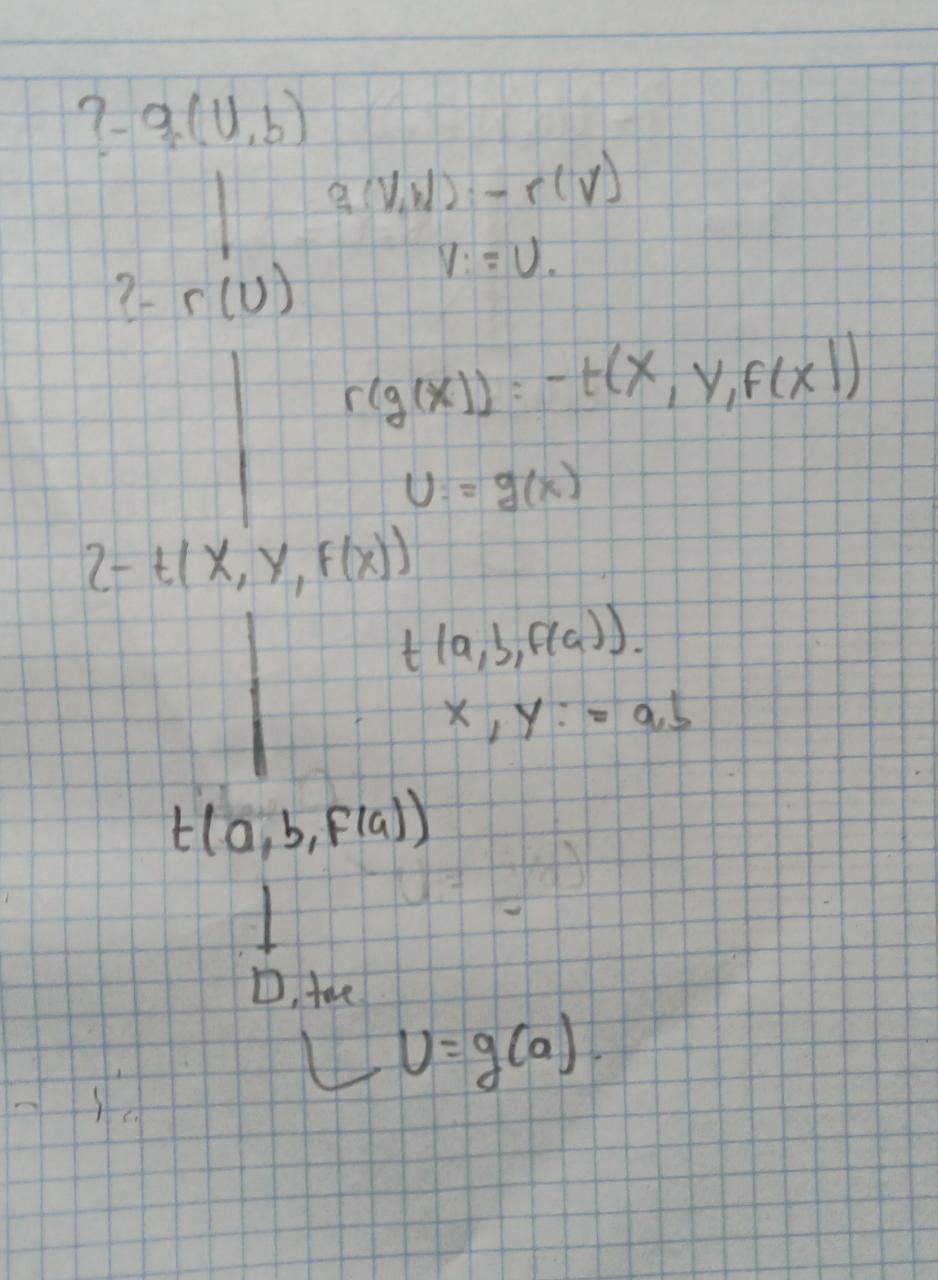
\includegraphics[scale=0.25]{E1}
  \end{center}
\item Muestra el árbol de búsqueda para la meta {\tt ?- t(a,W,f(V))}.

    \begin{center}
      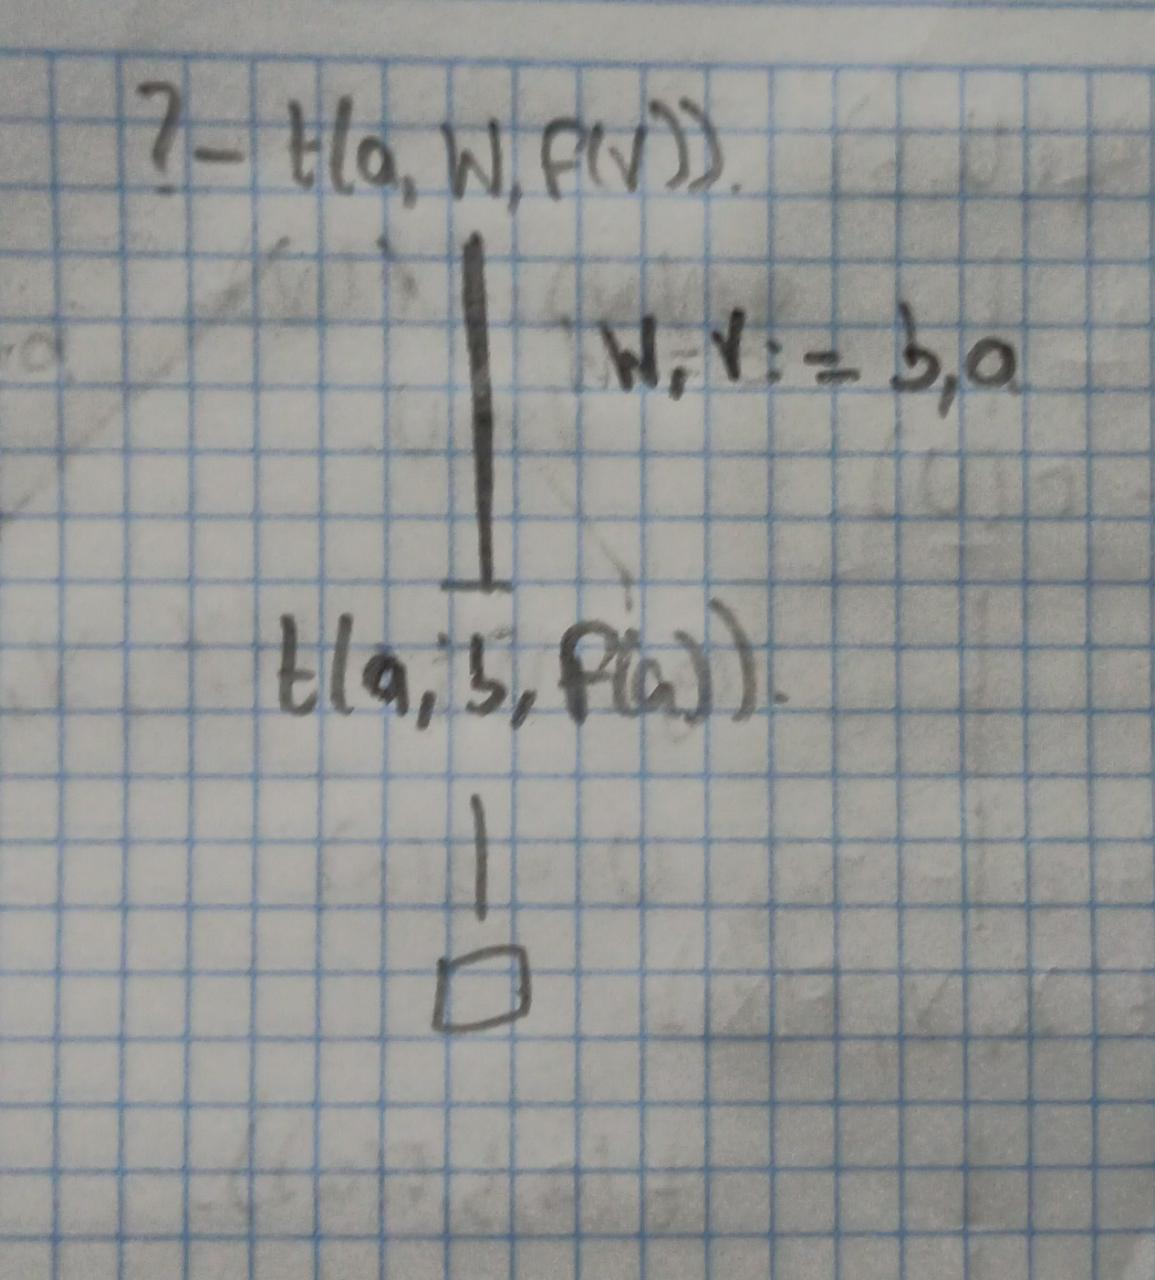
\includegraphics[scale=0.12]{E2}
    \end{center}
\end{enumerate}

\end{enumerate}


\end{document}
